\documentclass{beamer}
\usepackage{tcolorbox}
\usepackage{hyperref}
\usepackage{../../shared/notation/notation}
\usepackage{subfig}

%\beamerdefaultoverlayspecification{<+->}
% \newcommand{\data}{\mathcal{D}}
% \newcommand\Item[1][]{%
% 	\ifx\relax#1\relax  \item \else \item[#1] \fi
% 	\abovedisplayskip=0pt\abovedisplayshortskip=0pt~\vspace*{-\baselineskip}}

\graphicspath{ {imgs/} }

\usetheme{metropolis}           % Use metropolis theme


\title{Bias-Variance and Cross Validation}
\date{\today}
\author{Nipun Batra and teaching staff}
\institute{IIT Gandhinagar}
\begin{document}
	\maketitle

	\begin{frame}{A Question!}
	What would be the decision boundary of a decision tree classifier? 
		
	\begin{figure}
		\centering
	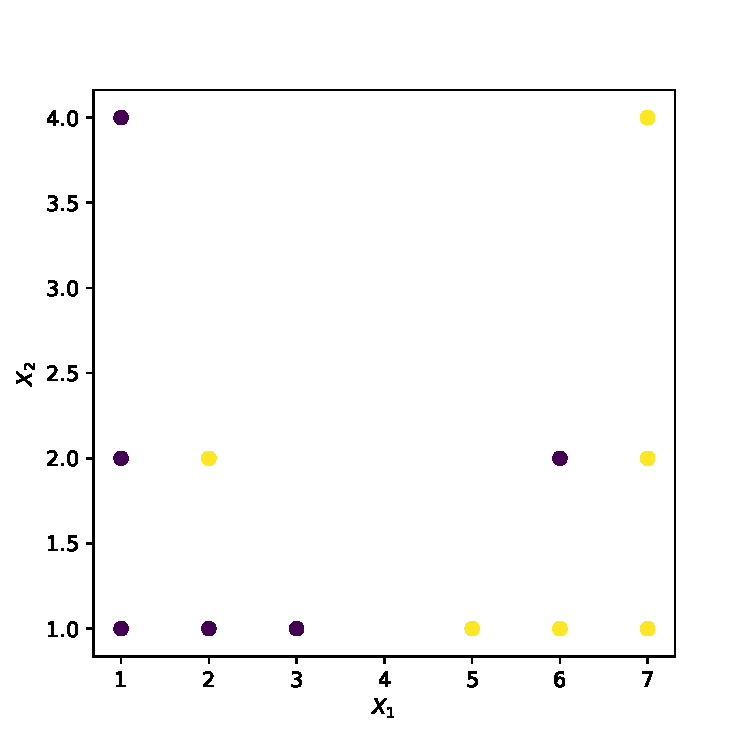
\includegraphics[scale=0.55]{dataset-1}
	\end{figure}


	\end{frame}

	\begin{frame}{Decision Boundary for a tree with depth 1}
	\begin{figure}%
	    \centering
	    \subfloat[Decision Boundary]{{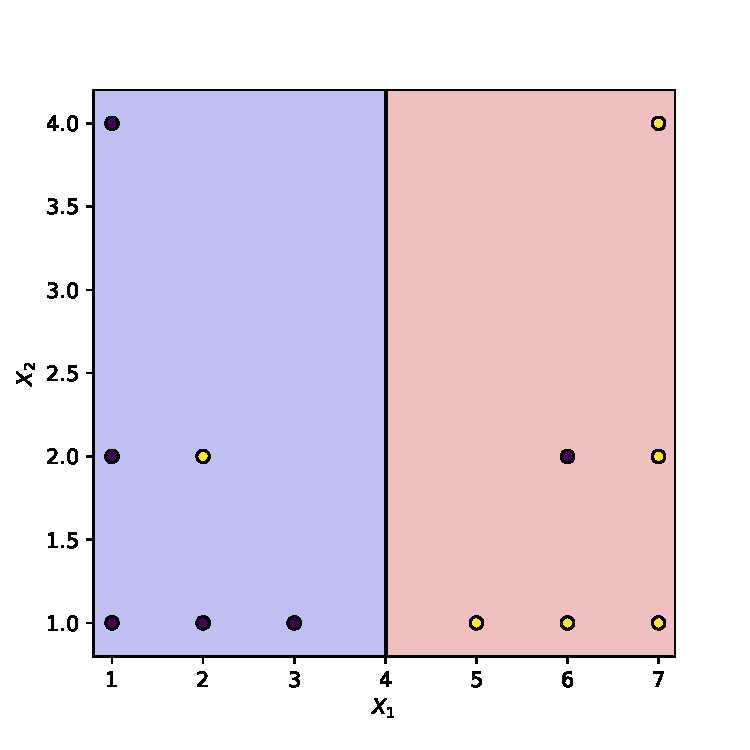
\includegraphics[width=0.45\textwidth]{example-1-depth-1-boundary} }}%
	    \qquad
	    \subfloat[Decision Tree]{{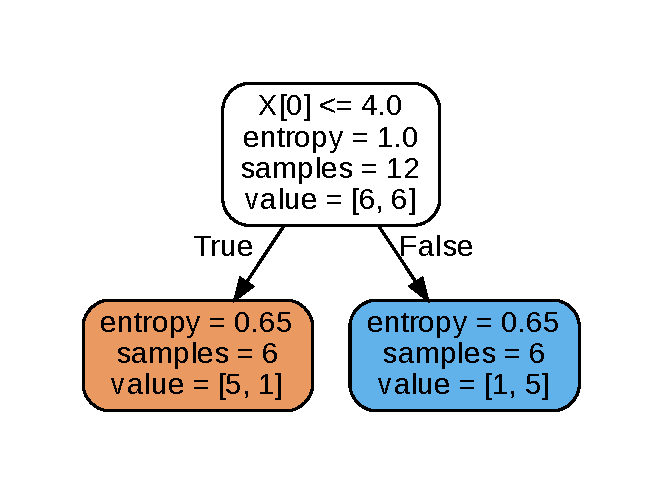
\includegraphics[width =0.45\textwidth]{example-1-depth-1-decision-tree} }}%
	    \label{fig:example}%
	\end{figure}
	\end{frame}
	
	\begin{frame}{Decision Boundary for a tree with no depth limit}
	\begin{figure}%
	    \centering
	    \subfloat[Decision Boundary]{{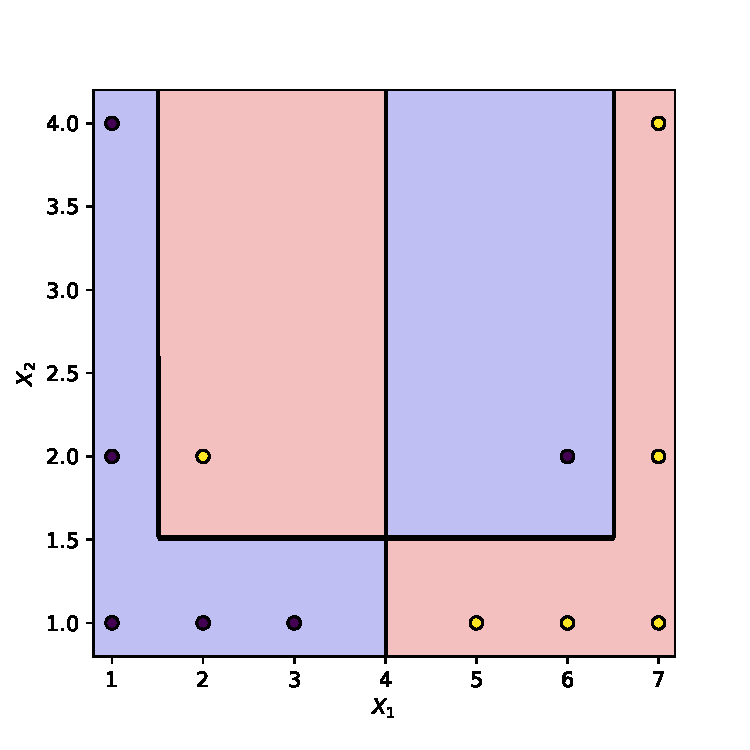
\includegraphics[width=0.45\textwidth]{example-1-nolimit-boundary} }}%
	    \qquad
	    \subfloat[Decision Tree]{{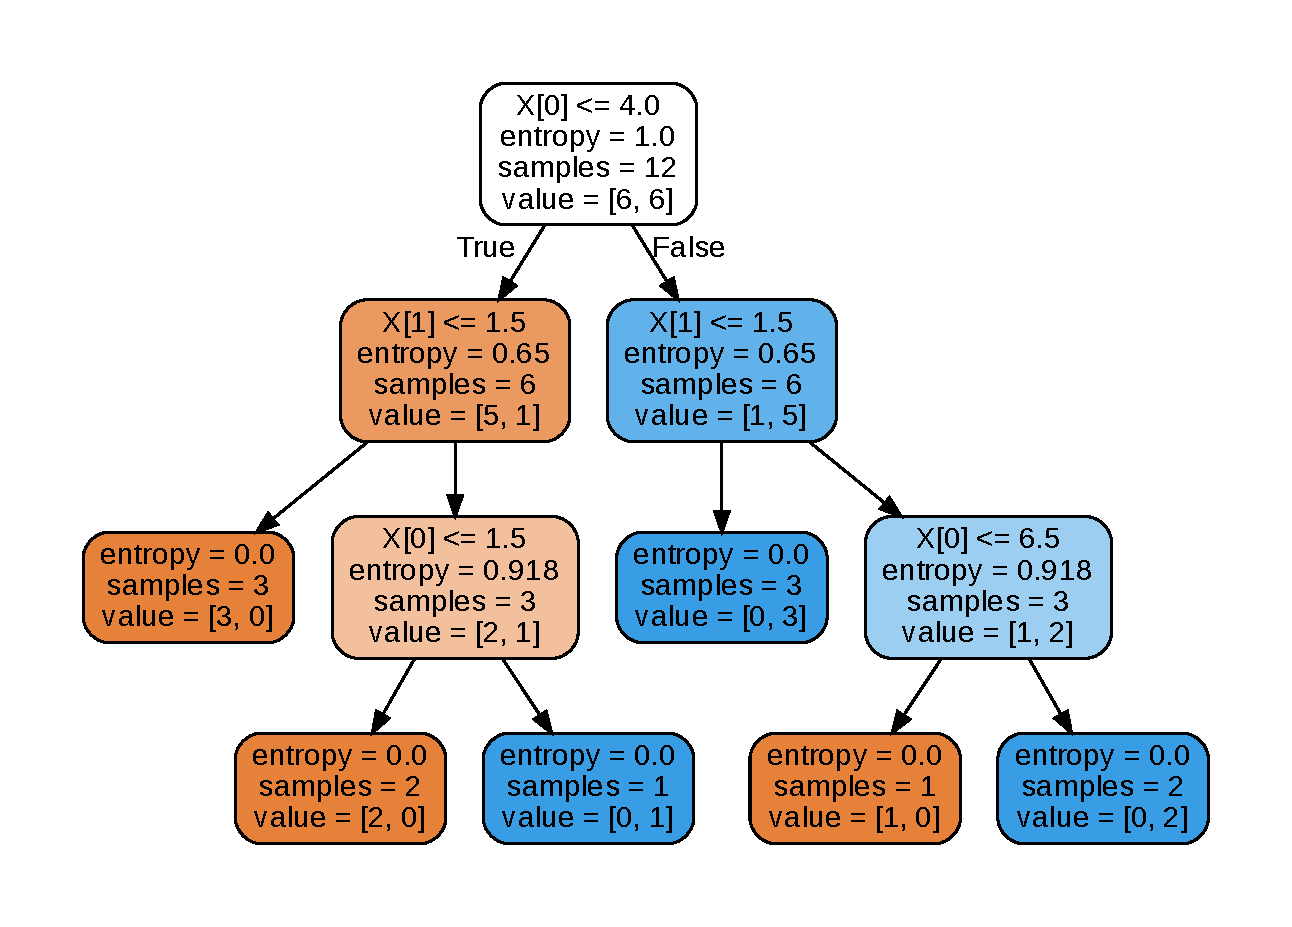
\includegraphics[width =0.45\textwidth]{example-1-nolimit-decision-tree} }}%
	    \label{fig:example}%
	\end{figure}
	\end{frame}
	

	\begin{frame}{Are deeper trees always better?}
	\only<1-2>{
	As we saw, deeper trees learn more complex decision boundaries.
	}
	
	\only<2>{
	\vspace{1cm}
	But, sometimes this can lead to $poor$ $generalization$
	}	
	\end{frame}

	\begin{frame}{An example}
	Consider the dataset below
	\begin{figure}%
	    \centering
	    \subfloat[Train Set]{{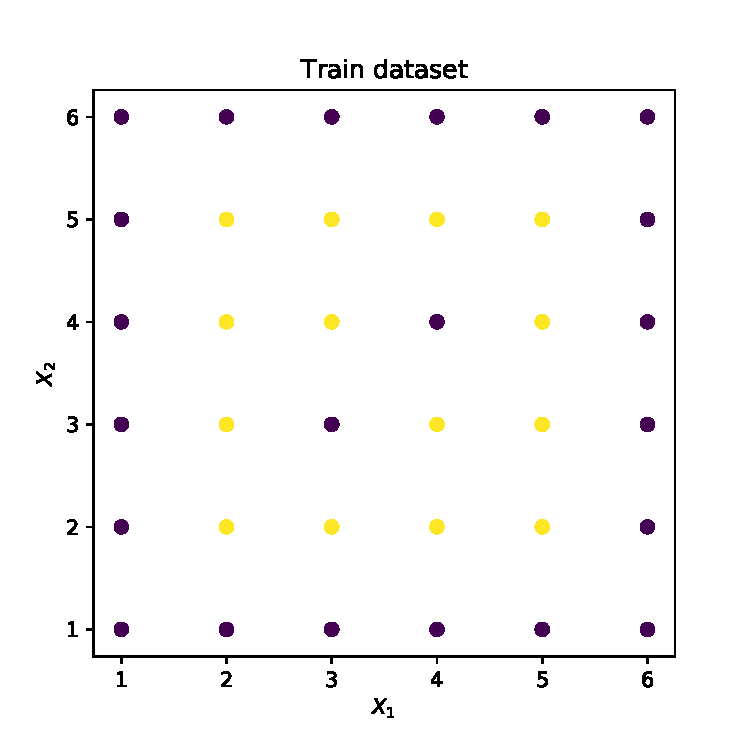
\includegraphics[width=0.45\textwidth]{dataset-2-train} }}%
	    \qquad
	    \subfloat[Test Set]{{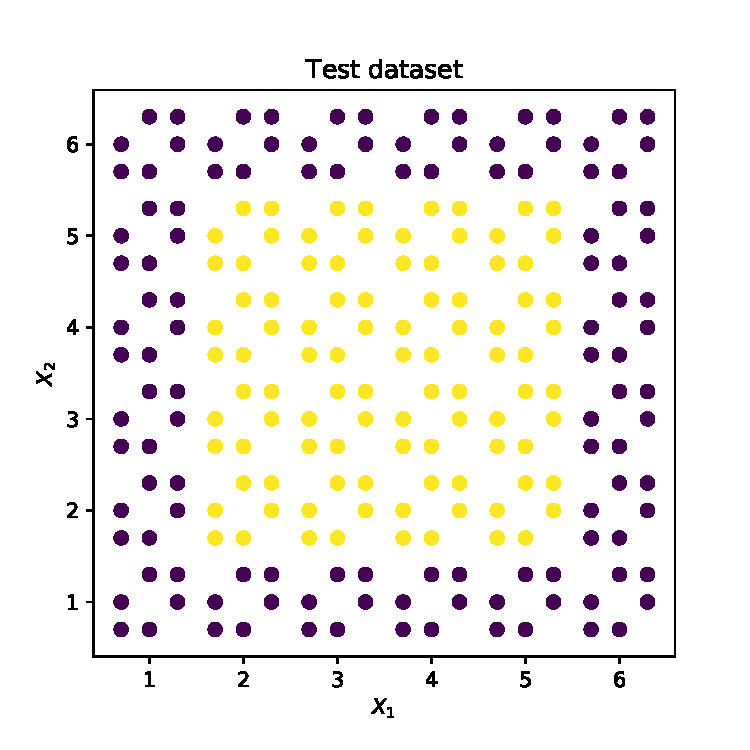
\includegraphics[width =0.45\textwidth]{dataset-2-test} }}%
	    \label{fig:example}%
	\end{figure}
	\end{frame}

	\begin{frame}{Underfitting}
	Underfitting is also known as $high$ $bias$, since it has a very biased incorrect assumption.
	\begin{figure}%
	    \centering
	    \subfloat[Decision Boundary]{{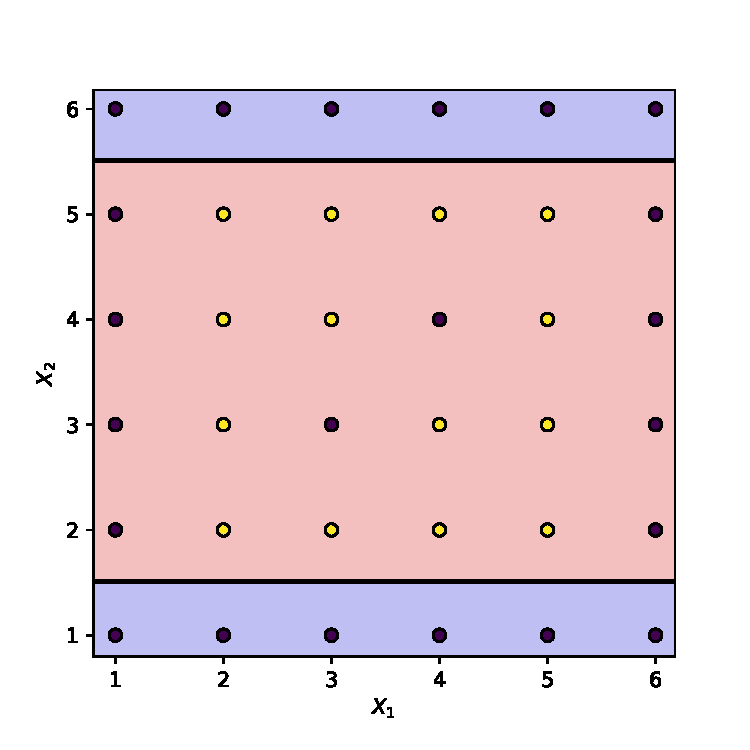
\includegraphics[width=0.45\textwidth]{example-2-depth-1-boundary} }}%
	    \qquad
	    \subfloat[Decision Tree]{{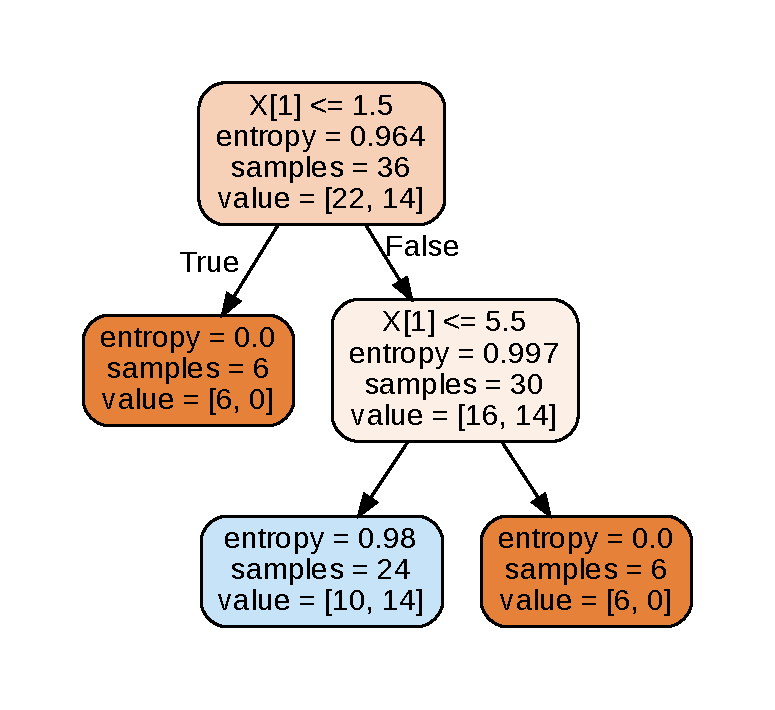
\includegraphics[width =0.45\textwidth]{example-2-depth-1-decision-tree} }}%
	    \label{fig:example}%
	\end{figure}
	\end{frame}

	\begin{frame}{Overfitting}
	Overfitting is also known as $high$ $variance$, since very small changes in data can lead to very different models.\\
	Decision tree learned has depth of 10.
	\begin{center}
	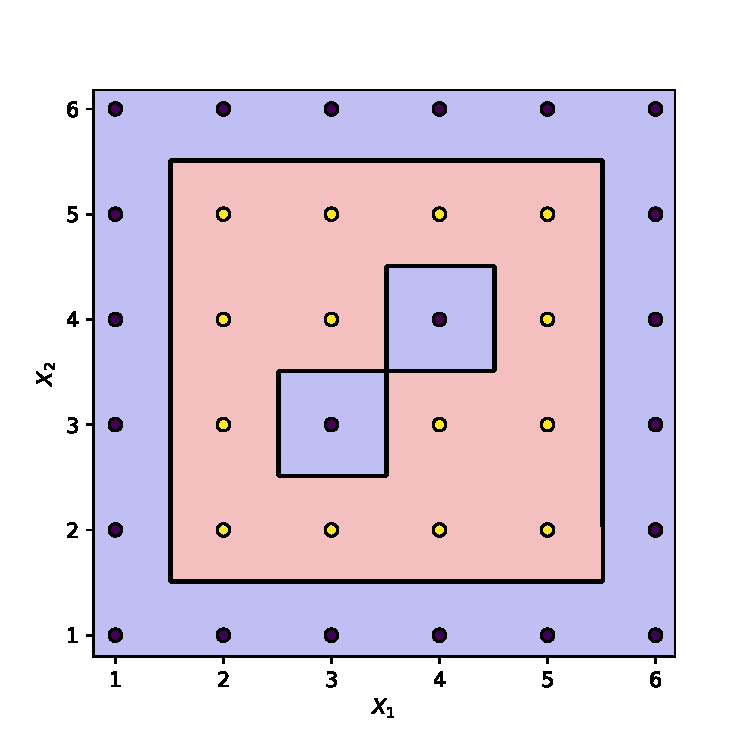
\includegraphics[scale=0.5]{example-2-nolimit-boundary}
	\end{center}
	\end{frame}


	\begin{frame}{Intution for Variance}
	A small change in data can lead to very different models.\\
	\vspace{1cm}
	\begin{columns}
		\begin{column}{0.5\textwidth}{\hspace{1.75cm} Dataset 1}
			\begin{center}
			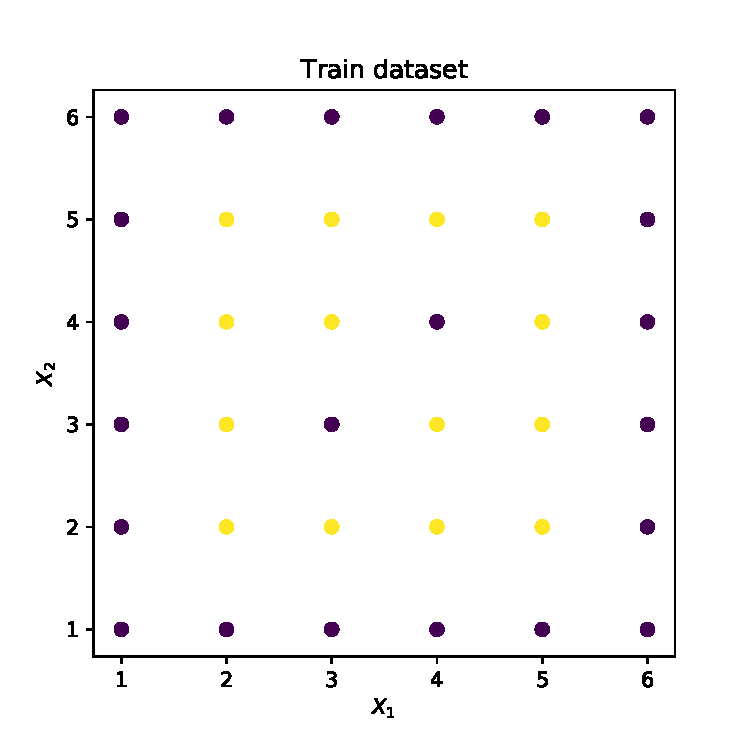
\includegraphics[width = \textwidth]{dataset-2-train}
			\end{center}
		\end{column}
		\begin{column}{0.5\textwidth}{\hspace{1.75cm} Dataset 2}
			\begin{center}
			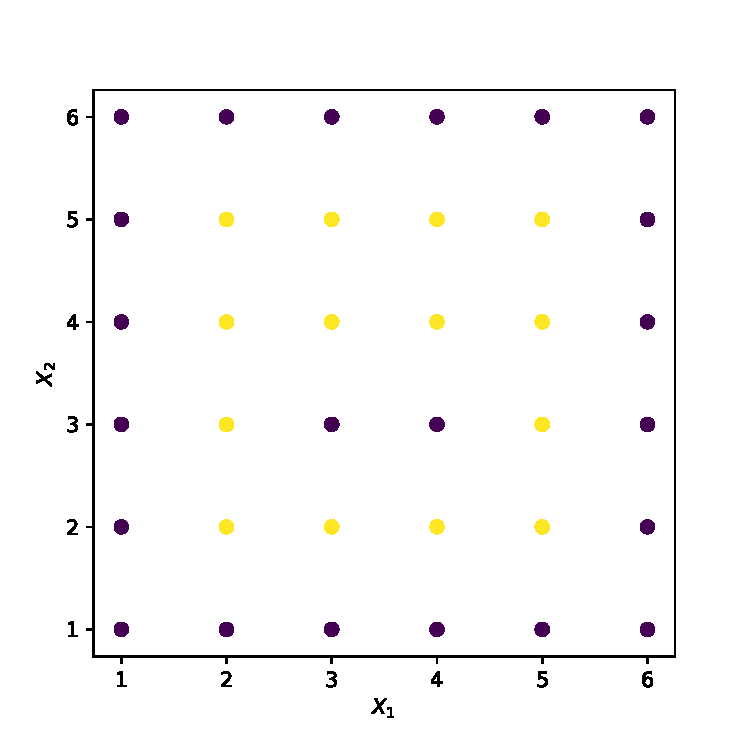
\includegraphics[width = \textwidth]{dataset-2-train-var}
			\end{center}
		\end{column}
	\end{columns}
	\end{frame}


	\begin{frame}{Intution for Variance}
	\begin{columns}
		\begin{column}{0.5\textwidth}
			\begin{center}
			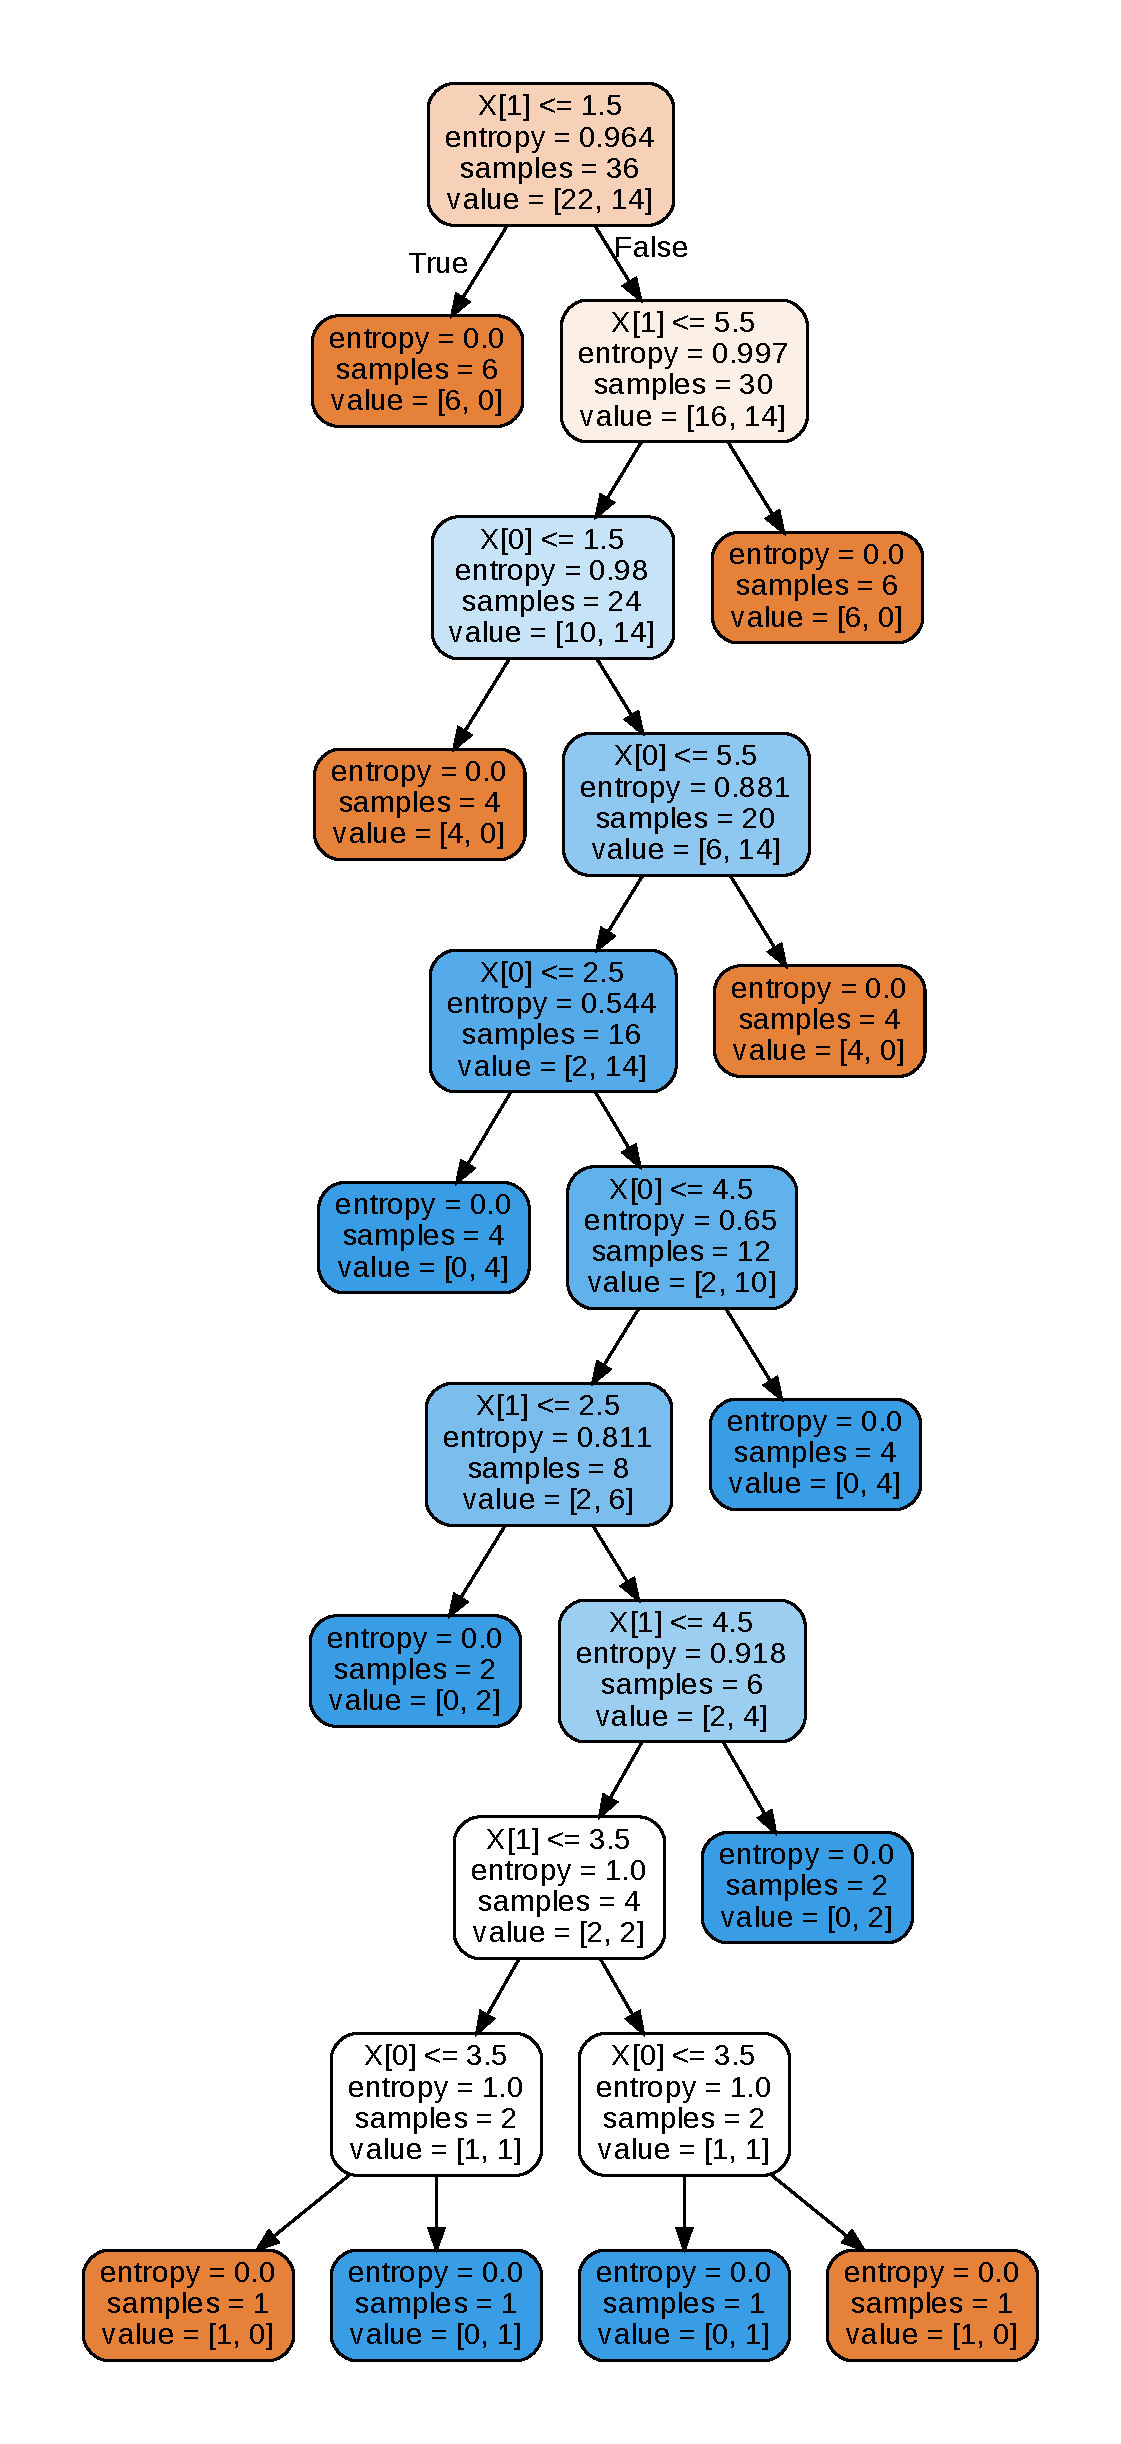
\includegraphics[scale=0.2]{var_1}
			\end{center}
		\end{column}
		\begin{column}{0.5\textwidth}
			\begin{center}
			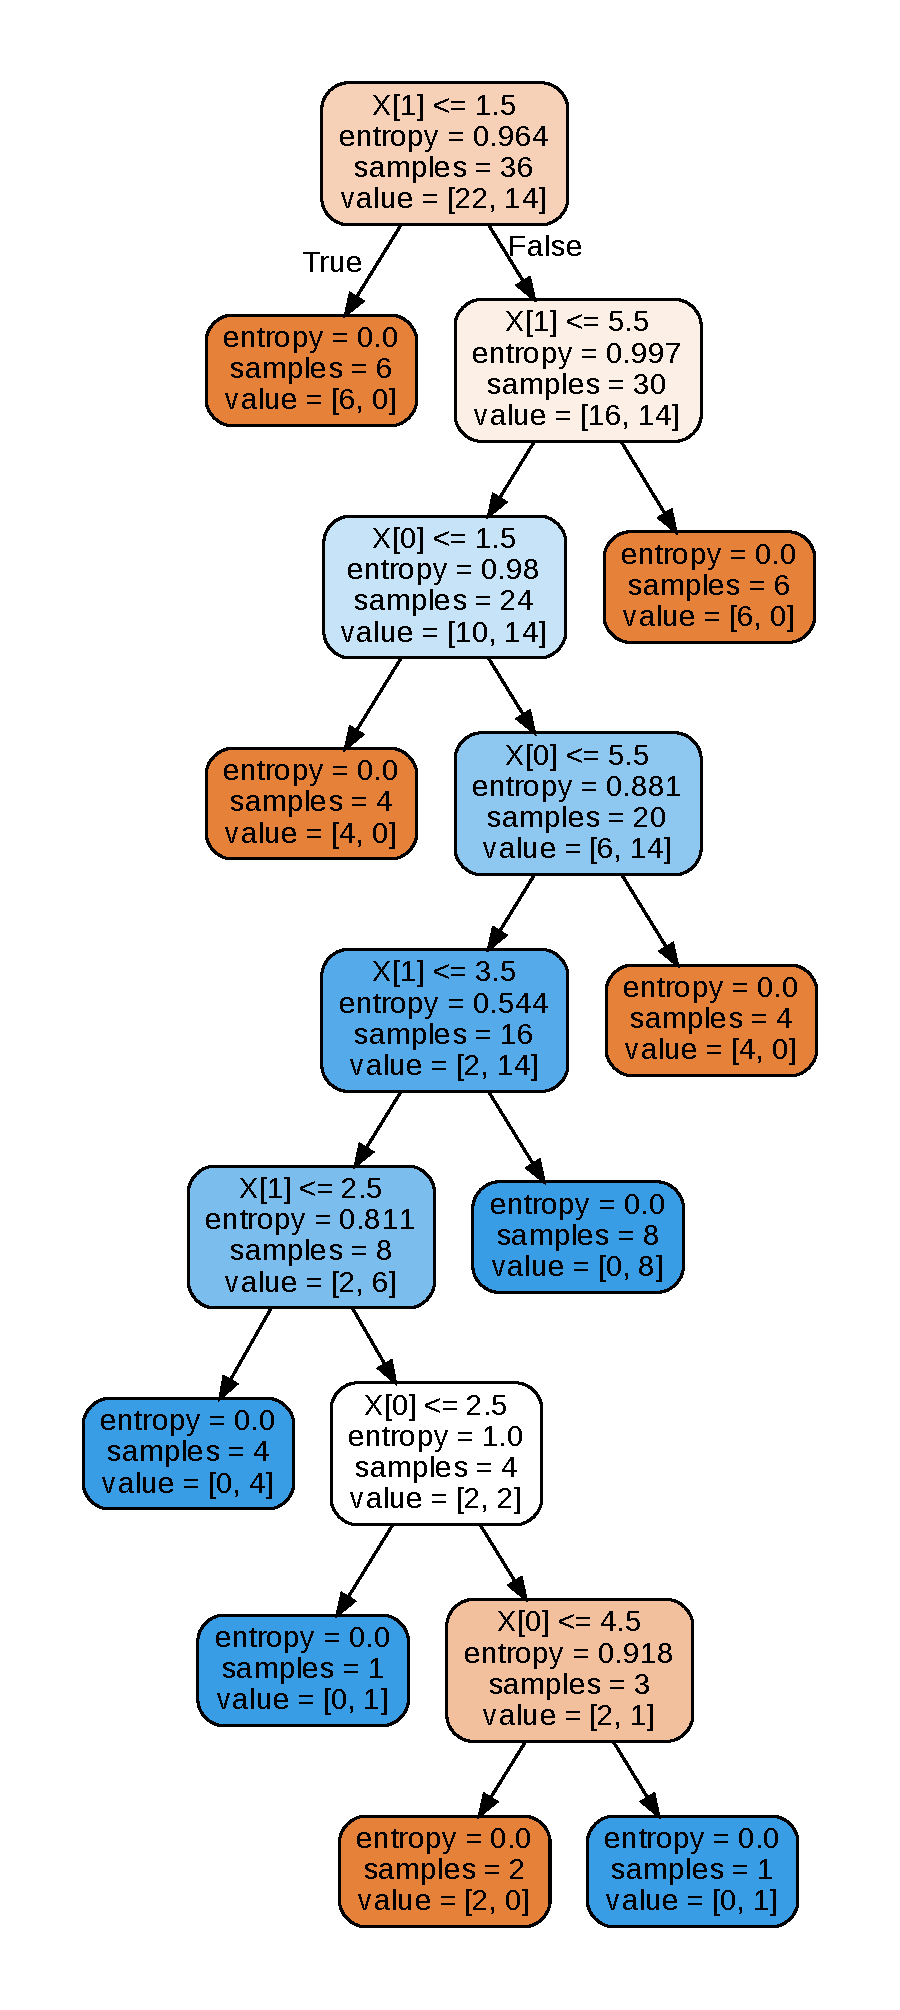
\includegraphics[scale=0.2]{var_2}
			\end{center}
		\end{column}
	\end{columns}
	\end{frame}


	\begin{frame}{A Good Fit}
	\begin{columns}
		\begin{column}{0.5\textwidth}
			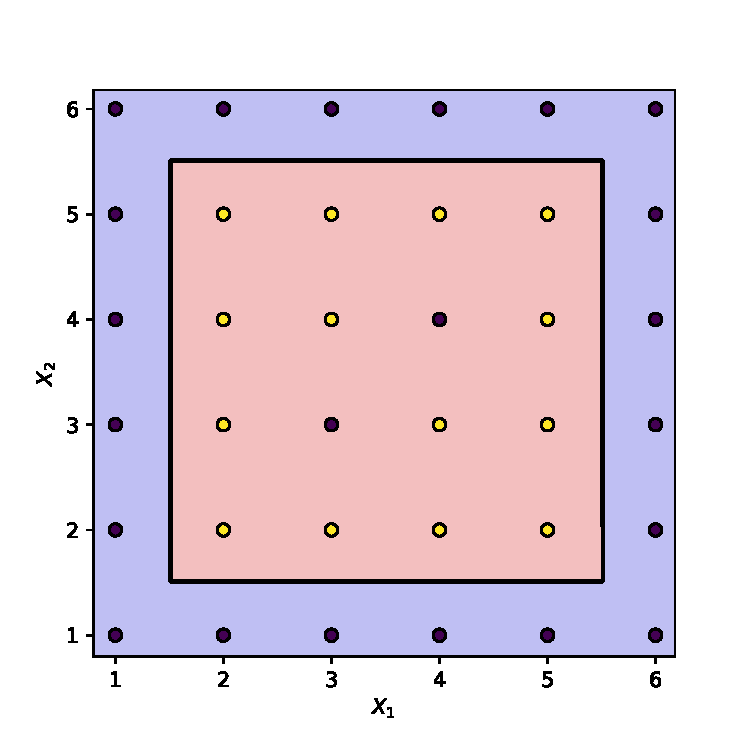
\includegraphics[width=\textwidth]{example-2-optimal-boundary}
		\end{column}
		\begin{column}{0.5\textwidth}
			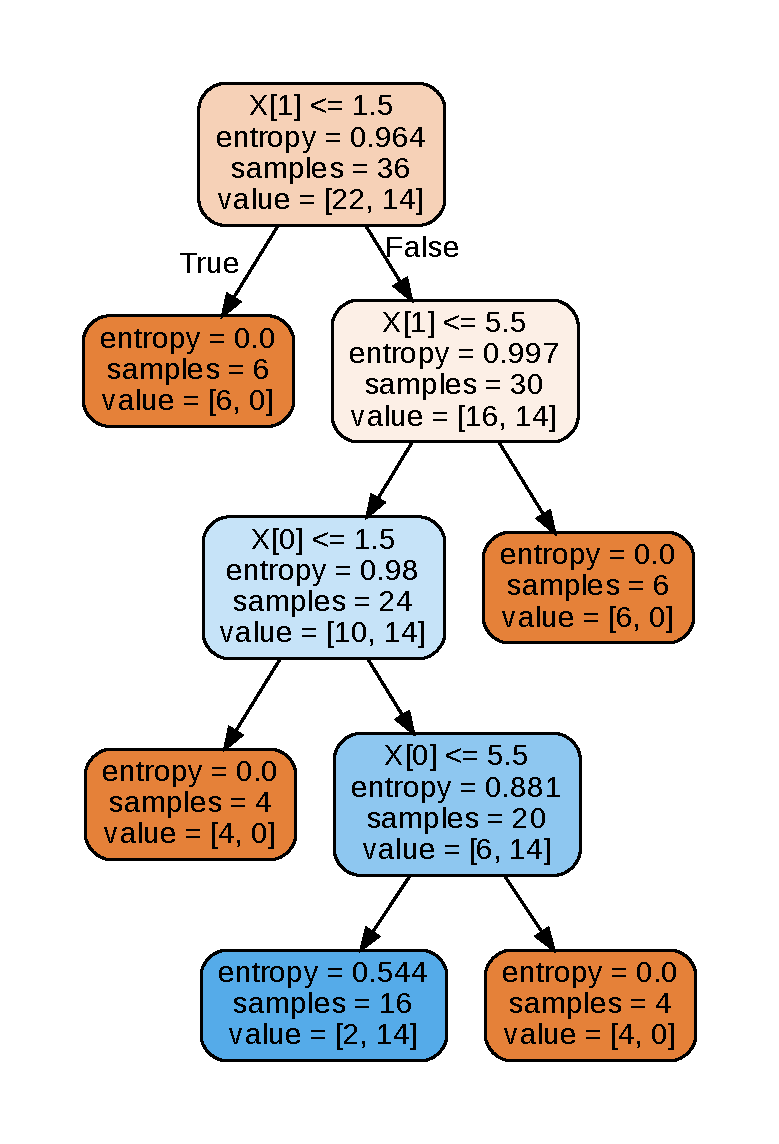
\includegraphics[width =\textwidth]{example-2-optimal-tree}
		\end{column}
	\end{columns}

	\end{frame}

	\begin{frame}{Accuracy vs Depth Curve}
		\begin{center}
		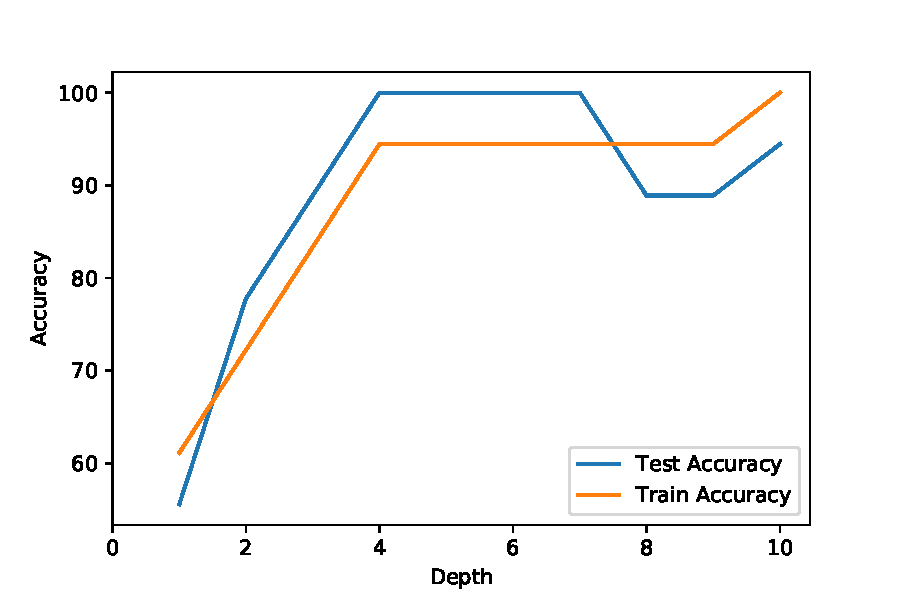
\includegraphics[scale=0.55]{acc-depth-plot}
	\end{center}
	\pause As depth increases, train accuracy improves\\
	\pause As depth increases, test accuracy improves till a point\\
	\pause At very high depths, test accuracy is not good (overfitting). 

	\end{frame}

	\begin{frame}{Accuracy vs Depth Curve : Underfitting}
	The highlighted region is the underfitting region.\\
	Model is too simple (less depth) to learn from the data. 
	\begin{center}
	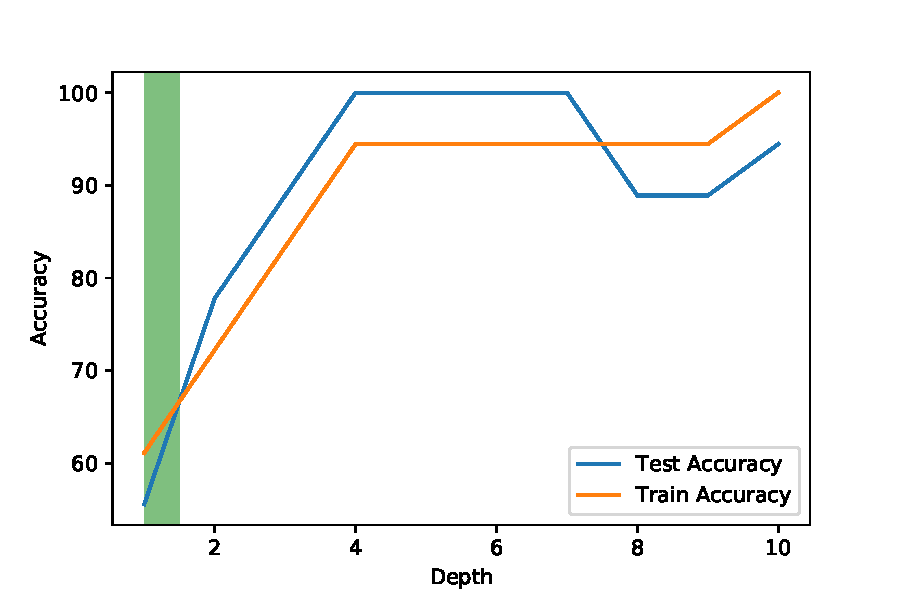
\includegraphics[scale=0.55]{acc-depth-plot-underfit}
	\end{center}
	\end{frame}

	\begin{frame}{Accuracy vs Depth Curve : Overfitting}
	The highlighted region is the overfitting region.\\
	Model is complex (high depth) and hence also learns the anomalies in data. 
	\begin{center}
	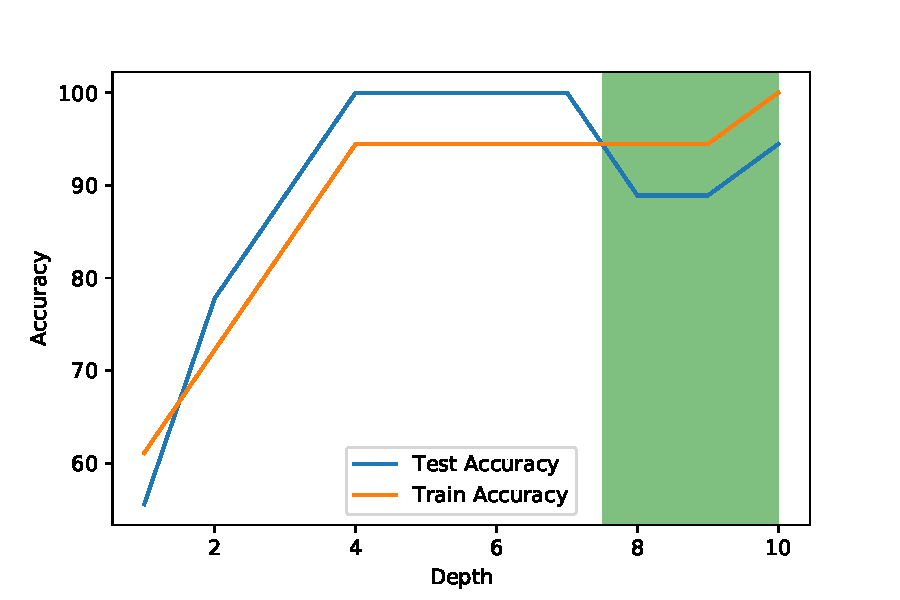
\includegraphics[scale=0.55]{acc-depth-plot-overfit}
	\end{center}
	\end{frame}

	\begin{frame}{Accuracy vs Depth Curve }
	The highlighted region is the good fit region.\\
	We want to maximize test accuracy while being in this region.
	\begin{center}
	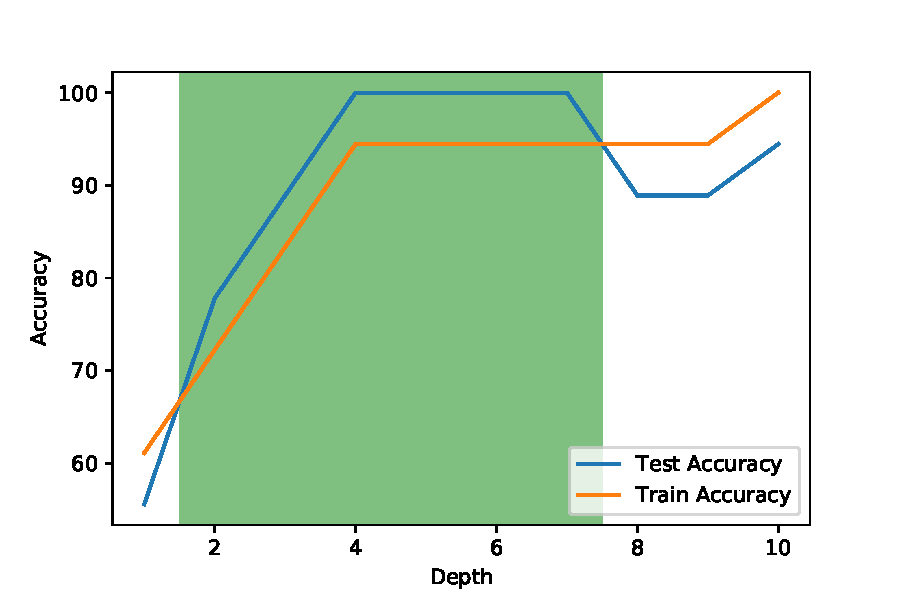
\includegraphics[scale=0.55]{acc-depth-plot-properfit}
	\end{center}
	\end{frame}

	\begin{frame}{The big question!?}
	\only<1-2>{
	How to find the optimal depth for a decision tree?\\
	}
	\only<2>{
	\vspace{1cm}
	Use cross-validation!
	}
	\end{frame}


	\begin{frame}{Our General Training Flow}
	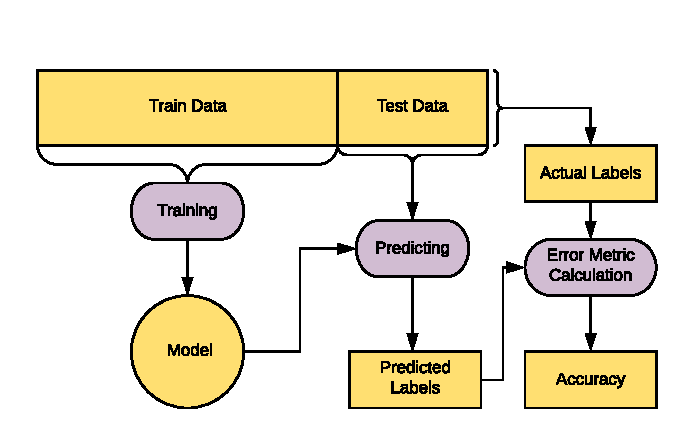
\includegraphics[width = \textwidth]{general-workflow}
	\end{frame}

	\begin{frame}{K-Fold cross-validation: Utilise full dataset for testing}
	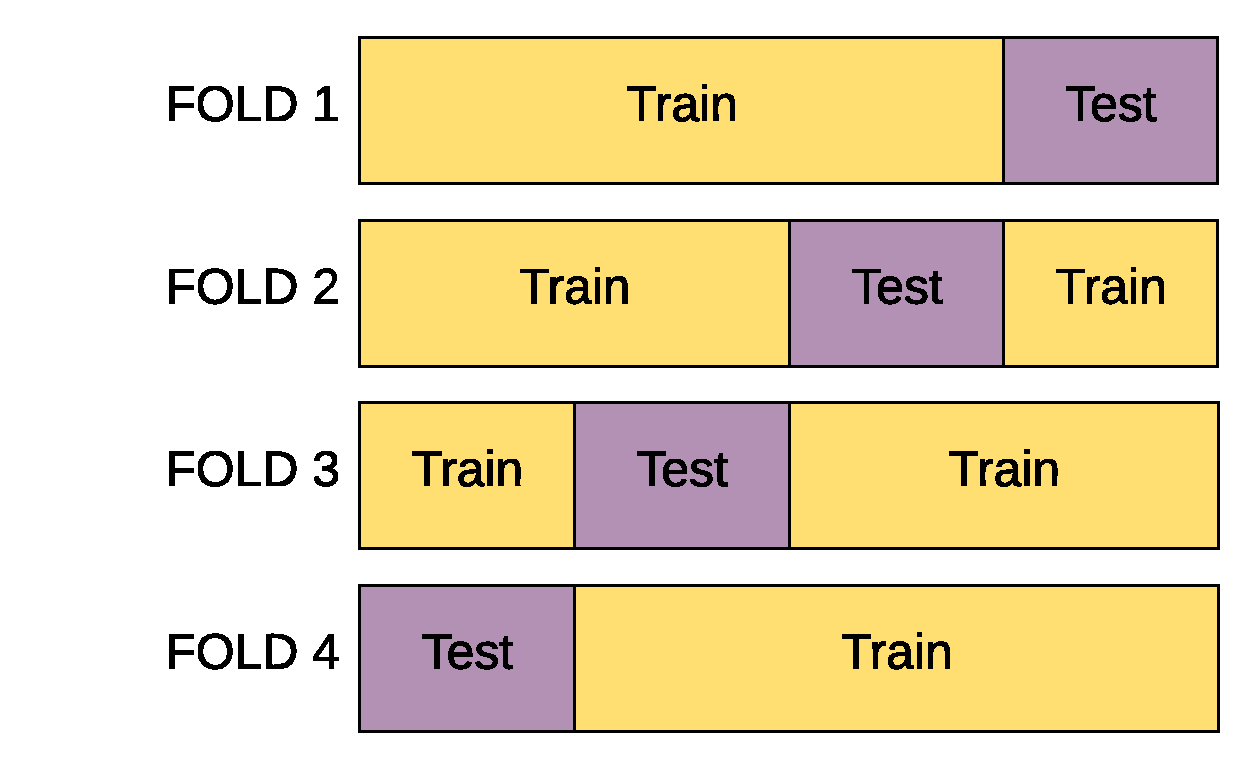
\includegraphics[width = \textwidth]{../cross-validation-train-test.pdf}
	\end{frame}

	\begin{frame}{The Validation Set}
	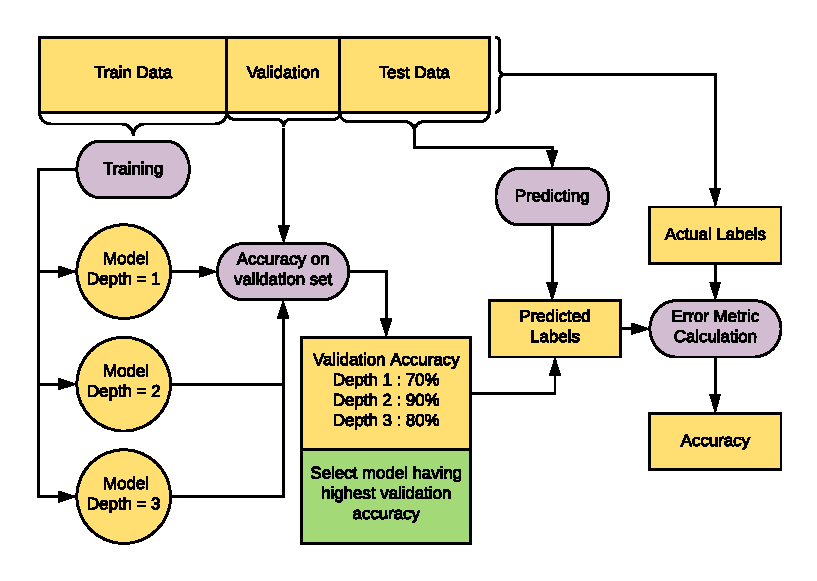
\includegraphics[width = \textwidth]{validation-workflow}
	\end{frame}

	\begin{frame}{Nested Cross Validation}
	Divide your training set into $K$ equal 	parts.\\
	 Cyclically use 1 part as ``validation set" and the rest for training.\\
	Here $K = 4$
	\begin{center}
	
\includegraphics[scale=0.7]{cross-validation}
	\end{center}
	\end{frame}

	\begin{frame}{Nested Cross Validation}
	Average out the validation accuracy across all the folds\\
	Use the model with highest validation accuracy\\
	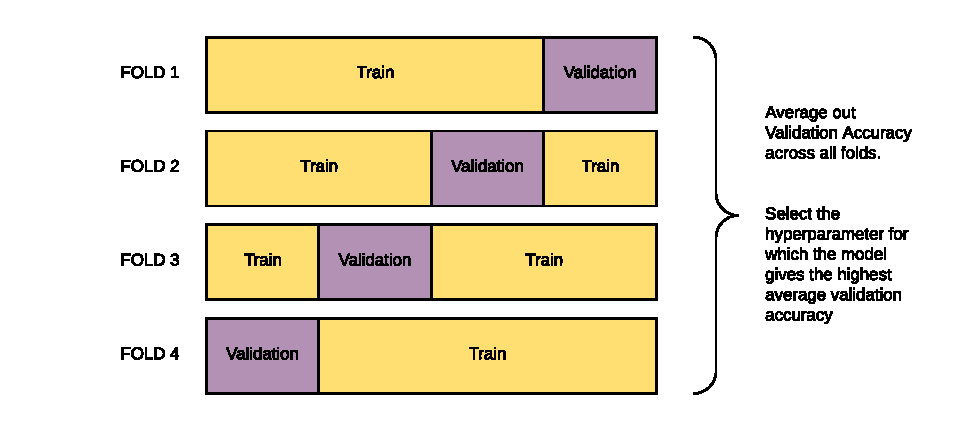
\includegraphics[width = \textwidth]{cross-validation-avg}
	\end{frame}

\begin{frame}{Next time: Ensemble Learning}
\begin{itemize}
	\item How to combine various models?
	\item Why to combine multiple models?
	\item How can we reduce bias?
	\item How can we reduce variance?
\end{itemize}
\end{frame}

%	\begin{frame}{Code for examples}
%	\begin{center}
%	\href{https://colab.research.google.com/drive/18E4HCN82GSa8-81h9yw2daHVg146IuWe}{Google Colab}
%	\end{center}
%	\end{frame}

\end{document}